% Options for packages loaded elsewhere
\PassOptionsToPackage{unicode}{hyperref}
\PassOptionsToPackage{hyphens}{url}
\PassOptionsToPackage{dvipsnames,svgnames,x11names}{xcolor}
%
\documentclass[
  letterpaper,
  DIV=11,
  numbers=noendperiod]{scrreprt}

\usepackage{amsmath,amssymb}
\usepackage{iftex}
\ifPDFTeX
  \usepackage[T1]{fontenc}
  \usepackage[utf8]{inputenc}
  \usepackage{textcomp} % provide euro and other symbols
\else % if luatex or xetex
  \usepackage{unicode-math}
  \defaultfontfeatures{Scale=MatchLowercase}
  \defaultfontfeatures[\rmfamily]{Ligatures=TeX,Scale=1}
\fi
\usepackage{lmodern}
\ifPDFTeX\else  
    % xetex/luatex font selection
\fi
% Use upquote if available, for straight quotes in verbatim environments
\IfFileExists{upquote.sty}{\usepackage{upquote}}{}
\IfFileExists{microtype.sty}{% use microtype if available
  \usepackage[]{microtype}
  \UseMicrotypeSet[protrusion]{basicmath} % disable protrusion for tt fonts
}{}
\makeatletter
\@ifundefined{KOMAClassName}{% if non-KOMA class
  \IfFileExists{parskip.sty}{%
    \usepackage{parskip}
  }{% else
    \setlength{\parindent}{0pt}
    \setlength{\parskip}{6pt plus 2pt minus 1pt}}
}{% if KOMA class
  \KOMAoptions{parskip=half}}
\makeatother
\usepackage{xcolor}
\setlength{\emergencystretch}{3em} % prevent overfull lines
\setcounter{secnumdepth}{5}
% Make \paragraph and \subparagraph free-standing
\ifx\paragraph\undefined\else
  \let\oldparagraph\paragraph
  \renewcommand{\paragraph}[1]{\oldparagraph{#1}\mbox{}}
\fi
\ifx\subparagraph\undefined\else
  \let\oldsubparagraph\subparagraph
  \renewcommand{\subparagraph}[1]{\oldsubparagraph{#1}\mbox{}}
\fi


\providecommand{\tightlist}{%
  \setlength{\itemsep}{0pt}\setlength{\parskip}{0pt}}\usepackage{longtable,booktabs,array}
\usepackage{calc} % for calculating minipage widths
% Correct order of tables after \paragraph or \subparagraph
\usepackage{etoolbox}
\makeatletter
\patchcmd\longtable{\par}{\if@noskipsec\mbox{}\fi\par}{}{}
\makeatother
% Allow footnotes in longtable head/foot
\IfFileExists{footnotehyper.sty}{\usepackage{footnotehyper}}{\usepackage{footnote}}
\makesavenoteenv{longtable}
\usepackage{graphicx}
\makeatletter
\def\maxwidth{\ifdim\Gin@nat@width>\linewidth\linewidth\else\Gin@nat@width\fi}
\def\maxheight{\ifdim\Gin@nat@height>\textheight\textheight\else\Gin@nat@height\fi}
\makeatother
% Scale images if necessary, so that they will not overflow the page
% margins by default, and it is still possible to overwrite the defaults
% using explicit options in \includegraphics[width, height, ...]{}
\setkeys{Gin}{width=\maxwidth,height=\maxheight,keepaspectratio}
% Set default figure placement to htbp
\makeatletter
\def\fps@figure{htbp}
\makeatother
% definitions for citeproc citations
\NewDocumentCommand\citeproctext{}{}
\NewDocumentCommand\citeproc{mm}{%
  \begingroup\def\citeproctext{#2}\cite{#1}\endgroup}
\makeatletter
 % allow citations to break across lines
 \let\@cite@ofmt\@firstofone
 % avoid brackets around text for \cite:
 \def\@biblabel#1{}
 \def\@cite#1#2{{#1\if@tempswa , #2\fi}}
\makeatother
\newlength{\cslhangindent}
\setlength{\cslhangindent}{1.5em}
\newlength{\csllabelwidth}
\setlength{\csllabelwidth}{3em}
\newenvironment{CSLReferences}[2] % #1 hanging-indent, #2 entry-spacing
 {\begin{list}{}{%
  \setlength{\itemindent}{0pt}
  \setlength{\leftmargin}{0pt}
  \setlength{\parsep}{0pt}
  % turn on hanging indent if param 1 is 1
  \ifodd #1
   \setlength{\leftmargin}{\cslhangindent}
   \setlength{\itemindent}{-1\cslhangindent}
  \fi
  % set entry spacing
  \setlength{\itemsep}{#2\baselineskip}}}
 {\end{list}}
\usepackage{calc}
\newcommand{\CSLBlock}[1]{\hfill\break\parbox[t]{\linewidth}{\strut\ignorespaces#1\strut}}
\newcommand{\CSLLeftMargin}[1]{\parbox[t]{\csllabelwidth}{\strut#1\strut}}
\newcommand{\CSLRightInline}[1]{\parbox[t]{\linewidth - \csllabelwidth}{\strut#1\strut}}
\newcommand{\CSLIndent}[1]{\hspace{\cslhangindent}#1}

\usepackage{fvextra}
\DefineVerbatimEnvironment{Highlighting}{Verbatim}{breaklines,commandchars=\\\{\}}
\DefineVerbatimEnvironment{OutputCode}{Verbatim}{breaklines,commandchars=\\\{\}}
\KOMAoption{captions}{tableheading}
\makeatletter
\@ifpackageloaded{tcolorbox}{}{\usepackage[skins,breakable]{tcolorbox}}
\@ifpackageloaded{fontawesome5}{}{\usepackage{fontawesome5}}
\definecolor{quarto-callout-color}{HTML}{909090}
\definecolor{quarto-callout-note-color}{HTML}{0758E5}
\definecolor{quarto-callout-important-color}{HTML}{CC1914}
\definecolor{quarto-callout-warning-color}{HTML}{EB9113}
\definecolor{quarto-callout-tip-color}{HTML}{00A047}
\definecolor{quarto-callout-caution-color}{HTML}{FC5300}
\definecolor{quarto-callout-color-frame}{HTML}{acacac}
\definecolor{quarto-callout-note-color-frame}{HTML}{4582ec}
\definecolor{quarto-callout-important-color-frame}{HTML}{d9534f}
\definecolor{quarto-callout-warning-color-frame}{HTML}{f0ad4e}
\definecolor{quarto-callout-tip-color-frame}{HTML}{02b875}
\definecolor{quarto-callout-caution-color-frame}{HTML}{fd7e14}
\makeatother
\makeatletter
\@ifpackageloaded{bookmark}{}{\usepackage{bookmark}}
\makeatother
\makeatletter
\@ifpackageloaded{caption}{}{\usepackage{caption}}
\AtBeginDocument{%
\ifdefined\contentsname
  \renewcommand*\contentsname{Table of contents}
\else
  \newcommand\contentsname{Table of contents}
\fi
\ifdefined\listfigurename
  \renewcommand*\listfigurename{List of Figures}
\else
  \newcommand\listfigurename{List of Figures}
\fi
\ifdefined\listtablename
  \renewcommand*\listtablename{List of Tables}
\else
  \newcommand\listtablename{List of Tables}
\fi
\ifdefined\figurename
  \renewcommand*\figurename{Figure}
\else
  \newcommand\figurename{Figure}
\fi
\ifdefined\tablename
  \renewcommand*\tablename{Table}
\else
  \newcommand\tablename{Table}
\fi
}
\@ifpackageloaded{float}{}{\usepackage{float}}
\floatstyle{ruled}
\@ifundefined{c@chapter}{\newfloat{codelisting}{h}{lop}}{\newfloat{codelisting}{h}{lop}[chapter]}
\floatname{codelisting}{Listing}
\newcommand*\listoflistings{\listof{codelisting}{List of Listings}}
\makeatother
\makeatletter
\makeatother
\makeatletter
\@ifpackageloaded{caption}{}{\usepackage{caption}}
\@ifpackageloaded{subcaption}{}{\usepackage{subcaption}}
\makeatother
\ifLuaTeX
  \usepackage{selnolig}  % disable illegal ligatures
\fi
\usepackage{bookmark}

\IfFileExists{xurl.sty}{\usepackage{xurl}}{} % add URL line breaks if available
\urlstyle{same} % disable monospaced font for URLs
\hypersetup{
  pdftitle={Data Literacy for the Language Sciences},
  pdfauthor={Elen Le Foll},
  colorlinks=true,
  linkcolor={blue},
  filecolor={Maroon},
  citecolor={Blue},
  urlcolor={Blue},
  pdfcreator={LaTeX via pandoc}}

\title{Data Literacy for the Language Sciences}
\usepackage{etoolbox}
\makeatletter
\providecommand{\subtitle}[1]{% add subtitle to \maketitle
  \apptocmd{\@title}{\par {\large #1 \par}}{}{}
}
\makeatother
\subtitle{A very gentle introduction to statistics and data
visualisation in R}
\author{Elen Le Foll}
\date{2024-04-20}

\begin{document}
\maketitle

\renewcommand*\contentsname{Table of contents}
{
\hypersetup{linkcolor=}
\setcounter{tocdepth}{2}
\tableofcontents
}
\bookmarksetup{startatroot}

\chapter*{Preface}\label{preface}
\addcontentsline{toc}{chapter}{Preface}

\markboth{Preface}{Preface}

\begin{tcolorbox}[enhanced jigsaw, rightrule=.15mm, bottomrule=.15mm, coltitle=black, breakable, toprule=.15mm, colbacktitle=quarto-callout-warning-color!10!white, titlerule=0mm, colframe=quarto-callout-warning-color-frame, colback=white, arc=.35mm, left=2mm, opacitybacktitle=0.6, opacityback=0, bottomtitle=1mm, leftrule=.75mm, title=\textcolor{quarto-callout-warning-color}{\faExclamationTriangle}\hspace{0.5em}{Warning}, toptitle=1mm]

This textbook draft is very much \textbf{work in progress}. I intend to
progressively add to it over the course of the summer semester 2024.

This first draft is intended as complementary materials to my summer
semester M.A.~class: ``More than counting words: Introduction to
statistics and data visualisation for linguists'' taught at the
University of Cologne.

Student feedback on this first draft is very welcome!

\end{tcolorbox}

\section*{Who is this book for?}\label{who-is-this-book-for}
\addcontentsline{toc}{section}{Who is this book for?}

\markright{Who is this book for?}

This textbook is intended as a very gentle introduction to basic
principles of data management, statistics, and data visualisation using
the programming language and environment `R`. The target audience are
students and researchers in the language sciences, including (applied)
linguistics, language teaching, and language education research. The
rationale for this textbook is based on my personal observations, in
teaching and consulting both students and researcher colleagues, that
many so-called `introductory' textbooks assume previous knowledge and
skills that all have or go through contents at too fast a pace for many
humanities scholars who often come with little to no experience with
programming and/or statistics.

The aim of this textbook is by no means to replace any of the brilliant
existing textbooks aimed at imparting statistical literacy for
linguistics research, but rather to provide a stepping stone towards
being able to make the most of these wonderful existing resources. A
(work-in-progress) list of next-step resources is included in
\href{https://elenlefoll.github.io/RstatsTextbook/FurtherResources.html}{Appendix
A}.

\begin{figure}[H]

{\centering 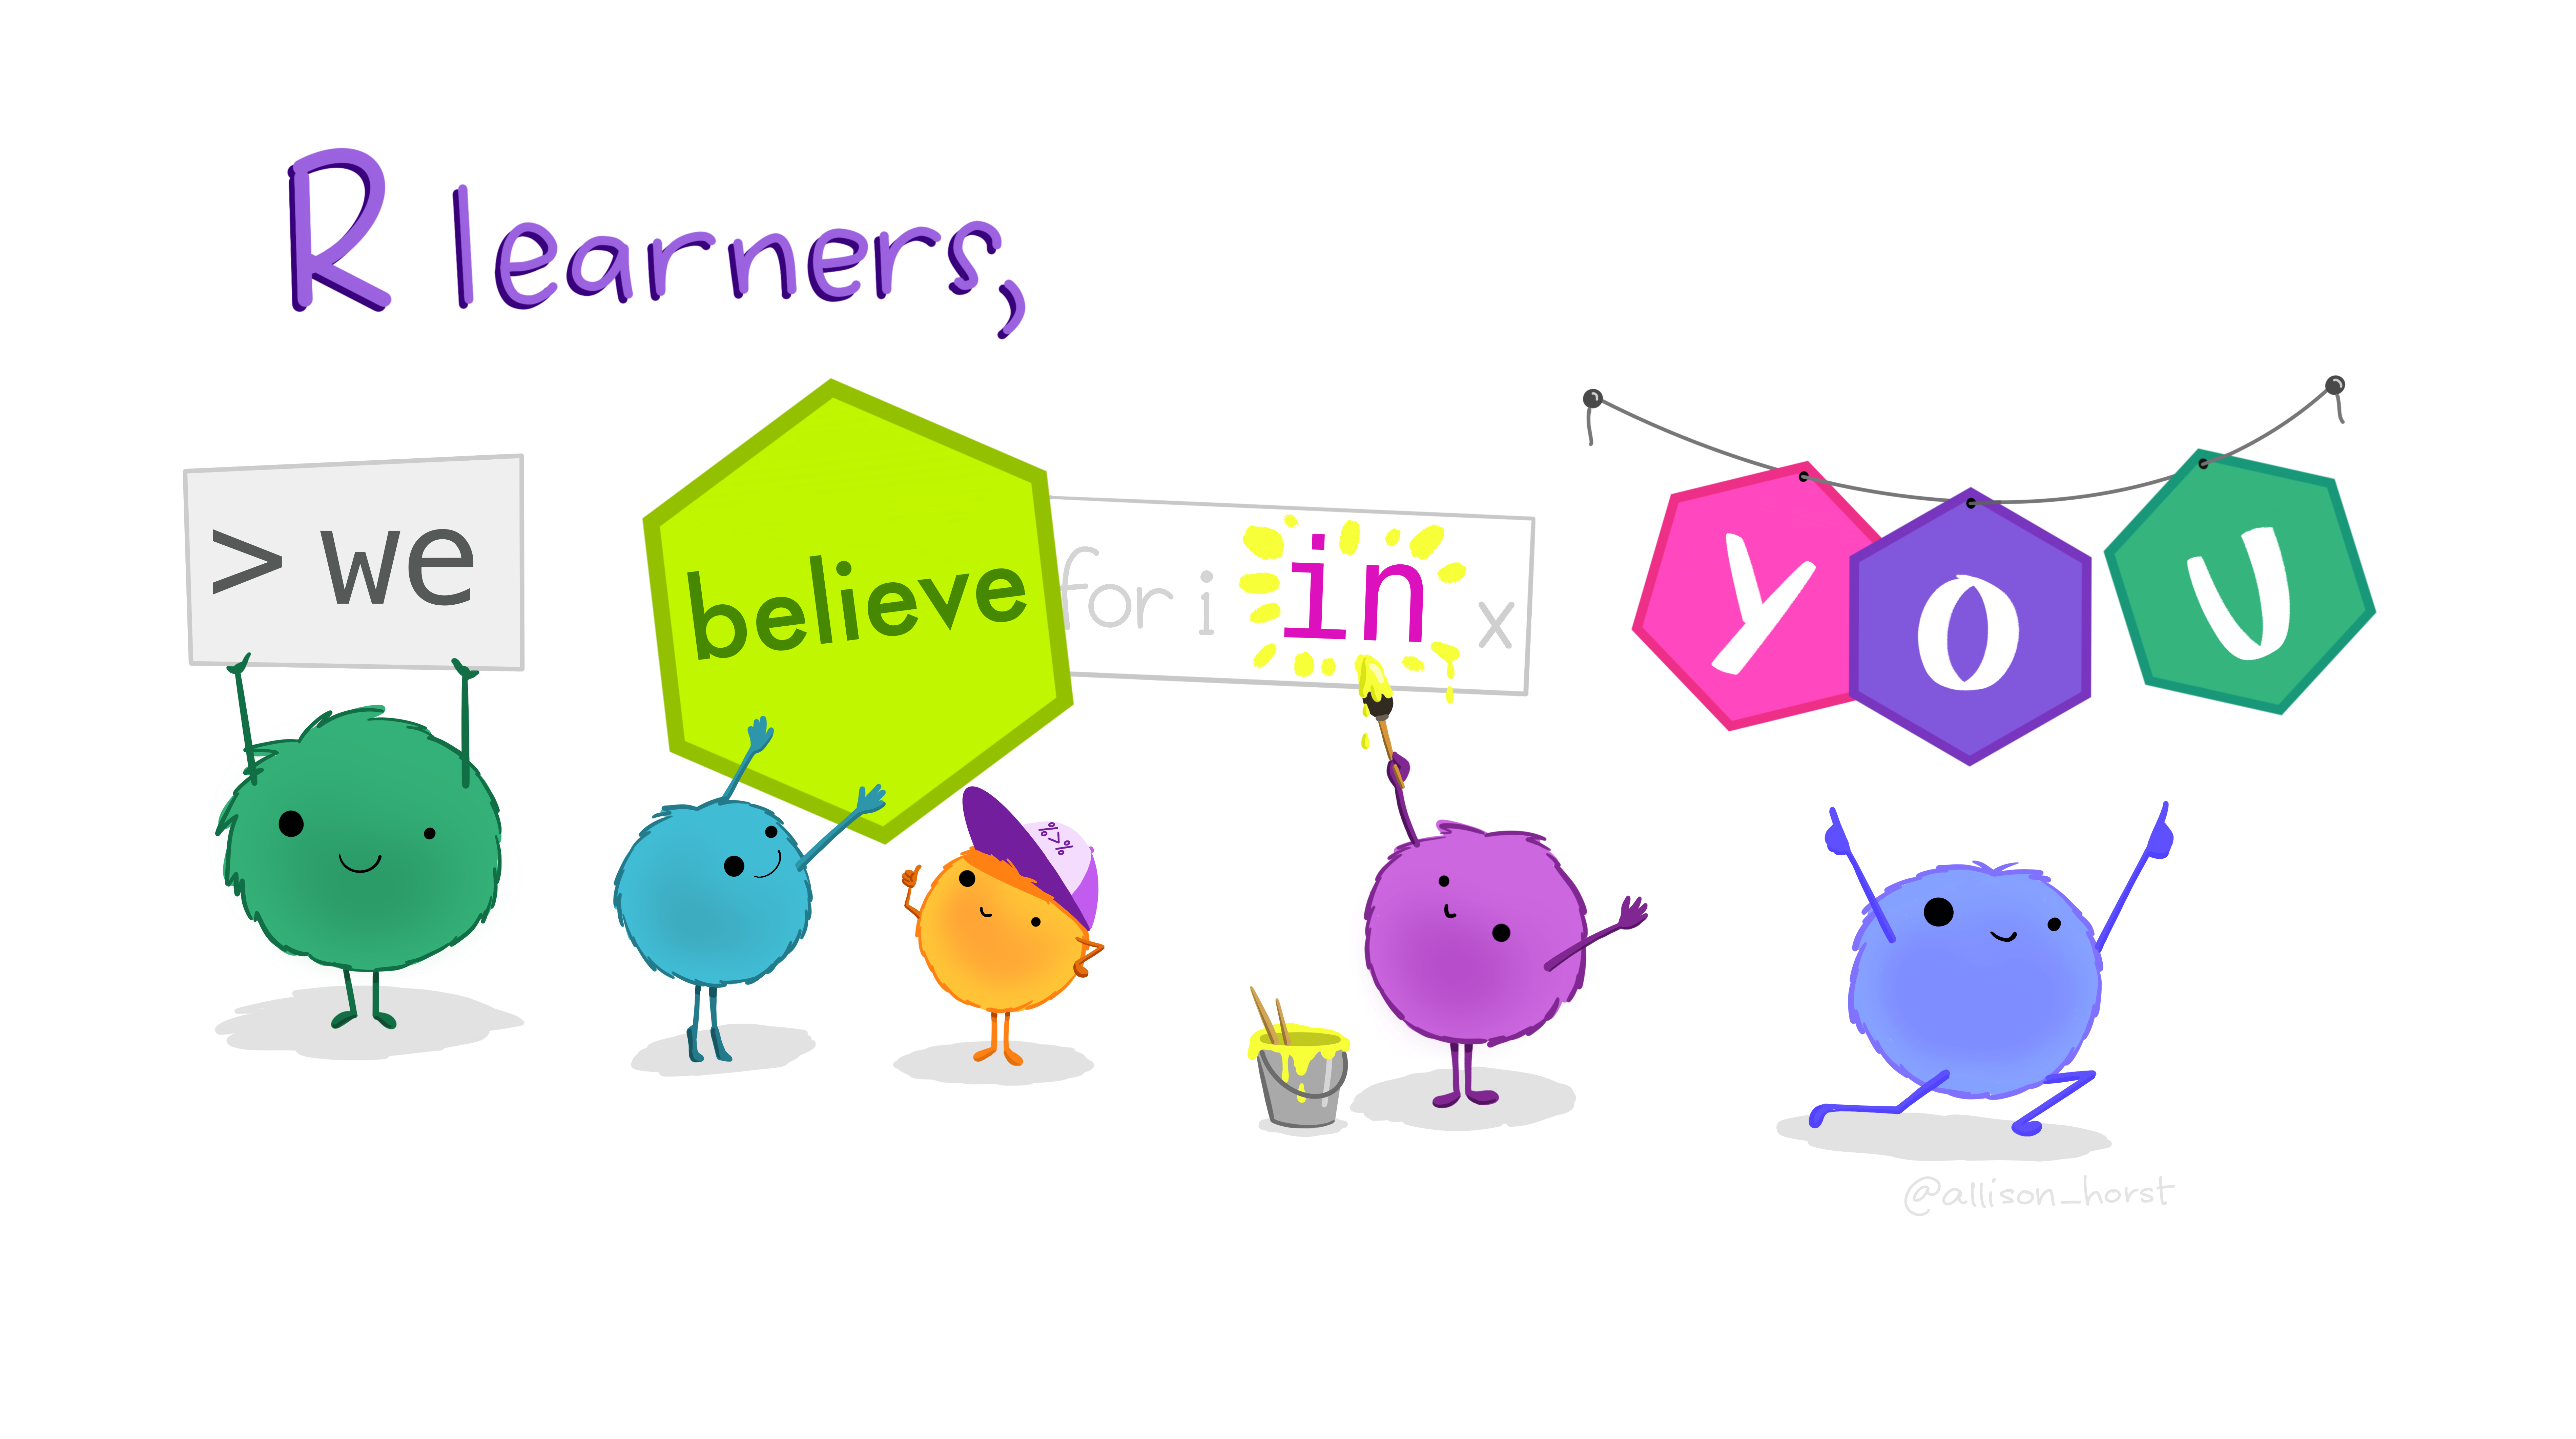
\includegraphics{images/RLearnersWeBelieve.png}

}

\caption{\emph{Artwork by @allison\_horst}}

\end{figure}%

\bookmarksetup{startatroot}

\chapter{Open Scholarship}\label{open-scholarship}

This book aims to provide a stepping stone for students and scholars of
traditionally less quantitative and computational disciplines (such as
some branches of linguistics and language education research) to gather
first (hopefully positive!) experiences with statistical and
computational approaches to working with empirical data\footnote{Emprical
  data is based on what is experienced or observed rather than on theory
  alone.}. The underlying belief is that these methods ought to be
accessible to all, regardless of their academic background or personal
circumstances. To this end, this book embraces the principles of Open
Scholarship.

Open Scholarship ``reflects the idea that knowledge of all kinds should
be openly shared, transparent, rigorous, reproducible, replicable,
accumulative, and inclusive (allowing for all knowledge systems)''
(Parsons et al. 2022). For this to be the case, teaching materials need
to shared openly and the tools and software taught in these resources
need to be freely accessible, too. In the following, we will briefly
consider the role of Open Educational Resources (OERs) and open-source
software in our pursuit of Open Scholarship.

\section{Open Source}\label{open-source}

In line with its aim to provide an accessible introduction to statistics
and data visualisation, this textbook relies exclusively on open-source
software and programming languages, foremost \texttt{LibreOffice\ Calc},
\texttt{R} and \texttt{RStudio}. Open source refers to software whose
source code is available under a license that grants anyone the rights
to study, modify, and distribute the software to anyone and for any
purpose. If we think of a software application as a cake, the source
code is like its recipe. It contains the list of ingredients and the
steps to bake the cake. Open source means that the recipe is publicly
available. You can access it, read it, and use it to bake the cake. You
can also modify it to add your own twist, such as adding a new
ingredient or making it vegan, and share it with others. In the context
of software, this allows many people to collaborate, make improvements,
and share their versions, resulting in better and more diverse software.

Using open-source software in this introductory textbook means that
anyone\footnote{Provided that they have access to the internet and a
  functioning personal computer.} can download, install and use the
required software at no cost. However, it is very important to note that
not all free software (\emph{freeware}) is open source. Let us
illustrate the difference by comparing different spreadsheet programmes
as, in the following chapter, we will begin exploring tabular data
structures in a spreadsheet programme.

The most most widely used spreadsheet programme to date is undoubtedly
\texttt{Microsoft\ Excel}. Excel is a commercial, proprietary
spreadsheet editor which forms part of the Microsoft 365 package. As
such, to use Excel on your personal computer, you need to buy a license
or be a member of an organisation (e.g., your university or company)
that pays for such a license. It is true that Microsoft now also offers
a free (functionally limited) web-based version of Excel, yet this still
does not make it open source. This is because Microsoft does not share
the source code of any Excel version, which means that, even if they are
giving away free cake, we do not have the recipe to bake the cake
ourselves should the company decide to start charging money for the cake
or to no longer distribute it at all! Similarly, you may be familiar
with a popular, web-based alternative to Excel: \texttt{Google\ Sheets}.
Whilst it is (currently) free to use, as the name suggests, Google
Sheets is owned by Google and is therefore not open source, either. By
contrast, \texttt{LibreOffice\ Calc} is a project of The Document
Foundation (TDF) that provides a popular, free, open-source office
productivity software suite comparable to Microsoft 365 called
\texttt{LibreOffice}. LibreOffice is developed collaboratively by very
many different people across the world who all do so on a volunteer
basis. The Document Foundation estimates that there are 200 million
active LibreOffice users worldwide, about 25\% of whom are thought to be
students (figures from 2018, see LibreOffice 2024). Its popularity is
likely due to the fact that it not only uses open formats (e.g.,
\texttt{.odt} and \texttt{.ods}), but can also open and save to a range
of popular formats including those used by Microsoft (e.g.,
\texttt{.docx} and \texttt{.xlsx}).

\begin{quote}
\section*{Quiz time!}\label{quiz-time}
\addcontentsline{toc}{section}{Quiz time!}

\markright{Quiz time!}

1) Which of these is an open-source alternative to Microsoft Word?

~

2) Which of these is an open-source alternative to Microsoft Powerpoint?

~

3) Not only can software be open source, programming languages can, too.
In fact, most modern programming languages are open source. In this
book, we will focus on the open-source programming language \texttt{R}.
Which of these is \emph{not} an open-source programming language?

~

4) There are also many open-source operating systems. Which of these is
an open-source alternative to the operating system Windows?

~
\end{quote}

\begin{tcolorbox}[enhanced jigsaw, rightrule=.15mm, bottomrule=.15mm, coltitle=black, breakable, toprule=.15mm, colbacktitle=quarto-callout-caution-color!10!white, titlerule=0mm, colframe=quarto-callout-caution-color-frame, colback=white, arc=.35mm, left=2mm, opacitybacktitle=0.6, opacityback=0, bottomtitle=1mm, leftrule=.75mm, title=\textcolor{quarto-callout-caution-color}{\faFire}\hspace{0.5em}{Task 1}, toptitle=1mm]

Your first task is to \textbf{download} and \textbf{install}
\textbf{LibreOffice} as we will use its spreadsheet editor,
\textbf{LibreOffice Calc}, in the next few chapters.

\begin{itemize}
\item
  LibreOffice is available for Windows, Mac and Linux. You can download
  it from here:
  \url{https://www.libreoffice.org/download/download-libreoffice/.}
\item
  You will find detailed installation instructions here:
  \href{https://www.libreoffice.org/get-help/install-howto/.You}{https://www.libreoffice.org/get-help/install-howto/.}
\item
  Detailed documentation is also available in many different languages:
  \url{https://documentation.libreoffice.org/en/english-documentation/}
\end{itemize}

\end{tcolorbox}

\section{Open Education}\label{open-education}

The web-based version of this textbook is published as an Open
Educational Resource (OER) under the Creative Commons license:
\href{https://creativecommons.org/licenses/by-nc-sa/4.0/}{\texttt{CC\ BY-NC-SA}}.
This means that it is free to read and use, as well as edit, remix, and
expand upon, provided that a) the original author and source is
mentioned (as indicated by
\href{https://creativecommons.org/licenses/by-nc-sa/4.0/}{\texttt{BY}}),
b) any derived version is not made into a commercial product
(\href{https://creativecommons.org/licenses/by-nc-sa/4.0/}{\texttt{NC}}
stands for non-commercial), and c) that any derived versions of this
textbook (e.g., a translated version or a version adapted for
historians) are also shared with this same license
(\href{https://creativecommons.org/licenses/by-nc-sa/4.0/}{\texttt{SA}}
stands for share alike).

In line with the principles of Open Education, all of the datasets that
we will work with in this textbook have been published in Open Access,
which means that we can freely use them to learn about statistics and
data visualisation using real datasets from published research studies
in applied linguistics and language education.

\begin{figure}[H]

{\centering 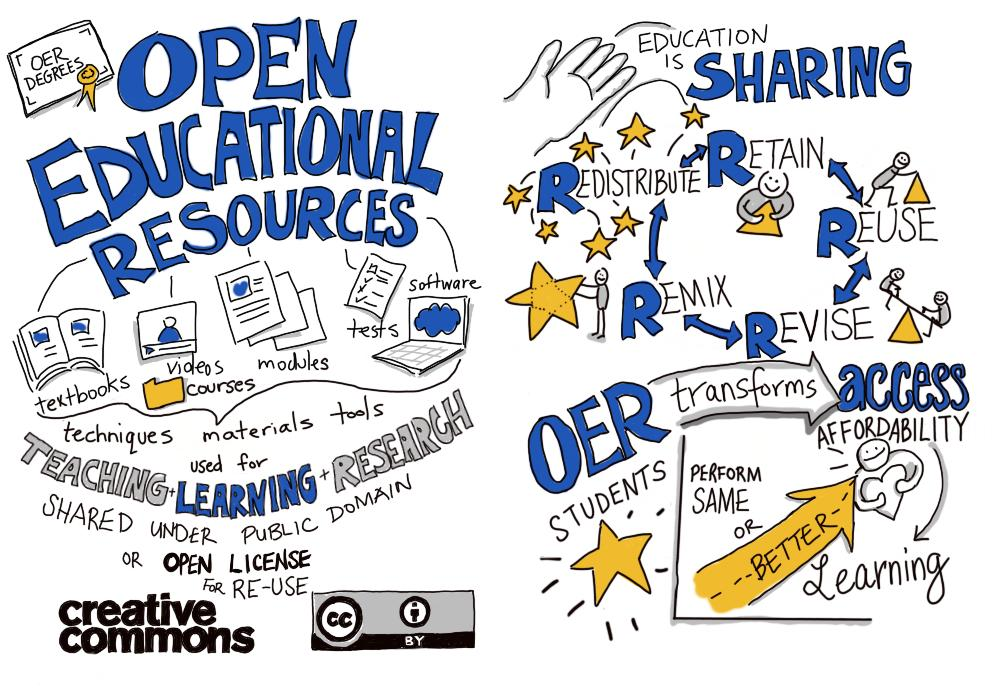
\includegraphics{images/oer.jpg}

}

\caption{OER sketch note by Yvonne Stry}

\end{figure}%

\begin{tcolorbox}[enhanced jigsaw, rightrule=.15mm, bottomrule=.15mm, coltitle=black, breakable, toprule=.15mm, colbacktitle=quarto-callout-note-color!10!white, titlerule=0mm, colframe=quarto-callout-note-color-frame, colback=white, arc=.35mm, left=2mm, opacitybacktitle=0.6, opacityback=0, bottomtitle=1mm, leftrule=.75mm, title=\textcolor{quarto-callout-note-color}{\faInfo}\hspace{0.5em}{Tips to go further}, toptitle=1mm]

This chapter has simplified things considerably. To be considered open
source, software distributions actually have to comply with ten
criteria. You can read up on them here:

\begin{itemize}
\tightlist
\item
  \url{https://opensource.org/osd}
\end{itemize}

To find out more about the benefits of open-source software in the
context of research, I recommend reading:

\begin{itemize}
\tightlist
\item
  \url{https://book.the-turing-way.org/reproducible-research/open/open-source}
\end{itemize}

To find out more about Open Educational Resources (OERs), I recommend
exploring the following OER databases:

\begin{itemize}
\item
  \url{https://oercommons.org/}
\item
  \url{https://www.twillo.de/oer/web/}
\end{itemize}

\end{tcolorbox}

\bookmarksetup{startatroot}

\chapter{Data}\label{data}

Most research in the language sciences is empirical, which means that it
is based on the analysis of data. But what kind of data are analysed in
(applied) linguistics and language education research?

\begin{tcolorbox}[enhanced jigsaw, rightrule=.15mm, bottomrule=.15mm, coltitle=black, breakable, toprule=.15mm, colbacktitle=quarto-callout-caution-color!10!white, titlerule=0mm, colframe=quarto-callout-caution-color-frame, colback=white, arc=.35mm, left=2mm, opacitybacktitle=0.6, opacityback=0, bottomtitle=1mm, leftrule=.75mm, title=\textcolor{quarto-callout-caution-color}{\faFire}\hspace{0.5em}{Task 1}, toptitle=1mm]

To find out more, visit the \href{https://iris-database.org/}{IRIS
website}. IRIS is a public, open repository where anyone can deposit the
data, materials, instruments, code, and tools that they used ``for
research into languages, including first, second, and beyond, and signed
language learning, multilingualism, language education, language use,
and language processing''. Go to its
\href{https://iris-database.org/search}{\texttt{Search\ and\ Download}}
page and scroll down to the filter option \texttt{Data\ Type} to get an
impression of the range of data types commonly used in language-related
research.

\begin{figure}[H]

{\centering 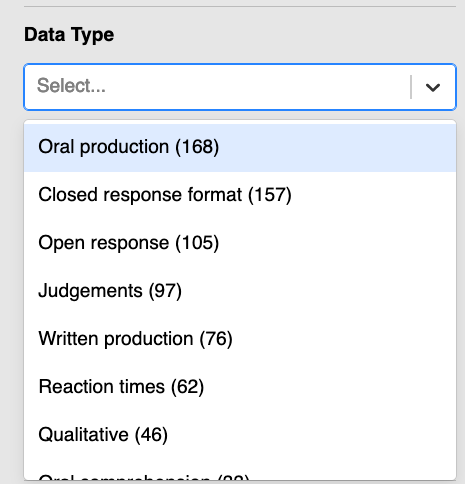
\includegraphics[width=2.60417in,height=\textheight]{images/IRISDataTypes.png}

}

\caption{\emph{Screenshot from the IRIS database search page (accessed
on 17 April 2024)}}

\end{figure}%

\end{tcolorbox}

\section{Types of data}\label{types-of-data}

Although the data types listed on the IRIS search page are very broad
and the categories not clearly defined, the list (see Fig. *) serves to
illustrate the breadth of research data types analysed in the language
sciences. The first category, `Oral production', for instance, could
equally refer to text transcriptions of language users' oral production,
audio, or video files. It could also either refer to raw data or to
(more or less) processed data. For example, a transcript of a
conversation could have been annotated for part-of-speech, meaning that
every word would be marked for their word class (e.g.,
\texttt{This\_DT\ is\_VBZ\ not\_RB\ raw\_JJ\ text\_NN\ data\_NN\ .\_PUNC}),
or it could include placeholders (e.g.,
\texttt{\textless{}proper\ noun\textgreater{}}) indicating that certain
words have been retracted for data protection reasons.

The category `Closed response format' includes all kinds of
questionnaires and tests. Questionnaires may ask study participants to
disclose personal information relevant to the research questions using
single or multiple-choice questions, such as what language they speak at
home, how long they have studied a language for, or how old they are.
Tests may be designed to assess participants' language competences
(e.g., in the form of a vocabulary or grammar test), as well as other
aspects relevant to the research questions being investigated (e.g.,
short-term memory or basic reaction times).

\section{Data formats}\label{data-formats}

Given the wide range of methods used in language research, there are
many different types of research data. Naturally, these come in various
data formats. For instance, audio files may be in \texttt{.wav} or
\texttt{.mp3} formats. Data may be collected with analogue means, e.g.,
by getting participants to answer a questionnaire on paper or collecting
learners' work on paper, but these data are typically digitalised for
analysis. They are then stored as text files in formats such as
\texttt{.txt} or \texttt{.csv}.

When researchers conduct an online survey, the data they collect is
typically stored in the form of tables.

But even if other data types are originally collected and/or analysed,
researchers will often end up doing their quantitative analyses on the
basis of tabular data. Consider a team of researchers going into schools
to investigate how foreign languages are taught and learnt in a specific
environment. They may record classroom interactions using video and
collect students' written work on paper. However, when it comes to the
quantitative data analysis, all of these data are likely to eventualy be
examined in the form of tables.

In the fieldwork research scenario, researchers may be interested in a
language community's use of a particular linguistic phenomenon, say
formal and informal forms of address. To this end, they obtain informed
consent from members of this community to record their interactions over
several weeks. The linguists will then transcribe their field
recordings. This allows them to search for the relevant forms of address
in the transcripts and, if necessary, to annotate the linguistic
features for various (e.g., socio-cultural) aspects. For the
quantitative data analysis, the forms of address and their associated
annotations would then be converted to a table format.

{[}Flowchart figure showing: picture of fieldwork with recording device
-\textgreater{} audio file -\textgreater{} text transcript
-\textgreater{} annotated text transcript -\textgreater{} data table{]}

\section{Working with tabular data}\label{working-with-tabular-data}

\begin{itemize}
\tightlist
\item
  Dangers of spreadsheet programmes
\item
  Specific problems of Excel!
\end{itemize}

\section{File management}\label{file-management}

\begin{verbatim}
- File naming
- File organisation
\end{verbatim}

\bookmarksetup{startatroot}

\chapter{Getting staRted in R}\label{getting-started-in-r}

\subsection{Chapter overview}\label{chapter-overview}

This chapter is designed to help you to get started using R and RStudio,
assuming no prior use of either.

We will be covering the following topics in this chapter:

\begin{itemize}
\tightlist
\item
  Downloading R and RStudio
\item
  Setting up RStudio
\item
  Writing and running code in RStudio
\end{itemize}

If you already have some experience of using R and RStudio, please
ensure that your R and RStudio versions are up-to-date. Whilst parts of
this chapter will likely be revision, others may be the opportunity to
learn some new tips about setting up and using R in RStudio. Once,
you've skimmed through this chapter, feel free to swiftly move on to the
next chapter.

\section{Why learn R?}\label{why-learn-r}

In short, because \texttt{R} can do it all! 🙃 This statement is only a
slight exaggeration: \texttt{R} is indeed a highly versatile programming
language and environment that allows you to do a multitude of tasks
relevant to the language sciences. These include data handling and
processing, statistical analysis, creating effective and appealing
(including interactive!) data visualisations, web scraping, text
analysis, generating reports in various formats, designing web pages and
interactive apps, and much, much more! 💪

Whilst some will claim that \texttt{R} has a steep learning curve, this
textbook aims to prove that the opposite is true! Whilst it's fair to
say that, as with all new things, it will take you a while to get the
hang of it, once you've got started, you will see that your
possibilities are endless and that learning how to do new things in
\texttt{R} is fun and very rewarding. This textbook introduces the
\{tidyverse\} approach to programming in R\texttt{,} which is very
accessible to beginners and we will use \texttt{RStudio} to work in
\texttt{R}, which also greatly facilitates the learning process.

What's more, both \texttt{R} and \texttt{RStudio} are free and open
source (see
\href{https://elenlefoll.github.io/RstatsTextbook/OpenScholarship.html}{Chapter
1}), which means that they are accessible to all, regardless of their
institutional affiliation or professional status. All you will need is
access to the internet, a computer, and the instrinsic motivation to
work your way through the basic skills taught in this textbook.

\begin{quote}
``{[}U{]}sing R - it's like the green and environment-friendly gardening
alternative to buying plastic wrapped tomatoes in the supermarket that
have no taste anyway.''
(\href{https://slcladal.github.io/whyr.html}{Martin Schweinberger 2022})

\begin{figure}

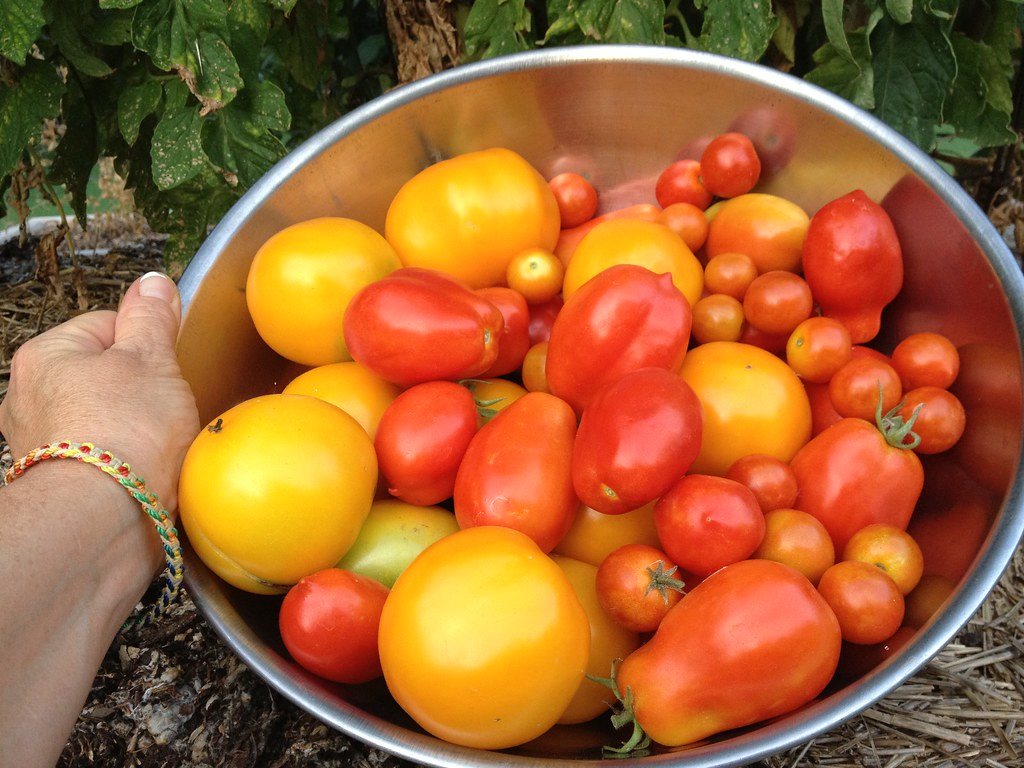
\includegraphics[width=3.91667in,height=\textheight]{images/TomatoHarvest.jpg}

\caption{\label{fig-tomatoes}``\href{https://www.flickr.com/photos/47264866@N00/9455141053}{Tomato
Harvest, Yellow \& Red}'' by
\href{https://www.flickr.com/photos/47264866@N00}{OakleyOriginals} is
licensed under
\href{https://creativecommons.org/licenses/by/2.0/?ref=openverse}{CC BY
2.0}.}

\end{figure}%
\end{quote}

Last but not least, in choosing to learn \texttt{R}, you are entering a
vibrant community of users. As an open-source programming environment,
\texttt{R} is the product of many different people's contributions.
Everyday, new packages, functions, and resources are being developed,
improved, and shared with the community. Given that \texttt{R} has
evolved into one of the most popular languages for scientific
programming (and is particularly popular among linguists, see e.g., ),
many of these have been created by scientists and are particularly
well-suited to research workflows. Moreover, the \texttt{R} community is
known for being welcoming, supportive, and inclusive (in contrast to
quite a few other communities in the computing world, sadly). This is
reflected in the strong presence of many community-led initiatives such
as \href{https://rladies.org/}{RLadies} and
\href{https://rainbowr.netlify.app/}{RainbowR}, which encourage
under-represented groups to participate in and contribute to the
\texttt{R} community.

\begin{figure}

\centering{


\includegraphics[width=2.13542in,height=\textheight]{images/rladiesrp_logo.png}

}

\caption{\label{fig-RLadies}Logo of the
\href{https://rladiesrp.github.io/}{RLadies Ribeirão Preto} meet-up
group, one of
\href{https://benubah.github.io/r-community-explorer/rladies.html}{many
RLadies chapters}.}

\end{figure}%

\subsection{\texorpdfstring{\emph{``Look, I am studying languages so why
should I learn to
code?''}}{``Look, I am studying languages so why should I learn to code?''}}\label{look-i-am-studying-languages-so-why-should-i-learn-to-code}

The main advantage of coding over using point-and-click tools (i.e.~GUI
{[}Graphical User Interface{]} software) is that everything single one
of your steps is recorded in the most precise way. Hence, your research
steps are entirely transparent and can be reproduced. Although this may
sound counter-intuitive, I can guarantee you that the person who will
benefit most from this is\ldots{} your future self! You will save a lot
of time and unnecessary headaches by being able to re-run your code,
rather than having to remember exactly what steps you took in each GUI
software and in what order. You will be far less likely to make mistakes
and, if you do, you will be able to correct them without fear of having
to redo all of your work. In other words, learn to use R will
considerably improve your research workflows from data processing to
data visualisation and reporting the results of your analyses. It will
reduce the risk for human errors, make your work more reproducible, and
help (future) you and others better understand how you processed and
analysed your data.

As we will see in a future chapter, \texttt{R} code is very easy to
export and share in various formats (including \texttt{.html} that can
be opened in any browser and \texttt{.pdf}). And because many other
language scientists use \texttt{R} too, you will also be able to share
your scripts with others, thus making your research more more
accessible, transparent, and sustainable and facilitating
collaborations. Being open-source, there are no restrictions as to who
can run \texttt{R} code and older versions are available ensuring that
exact reproduction is possible, even years later.

Learning to code in \texttt{R} is an excellent way to understand the
basics of data literacy and statistical reasoning. These are skills that
are highly valued among employers, both in academia and the industry.
Many companies, public institutions (e.g., ministries, hospitals, and
national agencies) and NGOs hire data scientists who often work in
\texttt{R}. And, even if you end up doing little to no coding yourself
later on, understanding the basic principles of programming is
undoubtedly a very useful skill in the modern world.

Some of you may be wondering whether you should be learning
\texttt{Python} rather than \texttt{R}. Both are widely used programming
languages in scientific programming and data science. However, there are
more resources specifically aimed at linguists and education researchers
in \texttt{R} than there are in Python simply because it is currently
the most widely used language in these disciplines. Should you wish to
learn \texttt{Python} at a later stage, many of the same principles that
you will have learned in \texttt{R} will apply: it should feel somewhat
like learning Italian when you already speak Spanish or French fluently.

\section{Installing R and RStudio}\label{installing-r-and-rstudio}

\subsection{What are R and RStudio? And why do I need
both?}\label{what-are-r-and-rstudio-and-why-do-i-need-both}

As a beginner, it's easy to confuse \texttt{R} and \texttt{RStudio}, but
it's important to understand that they are two very different things.
\texttt{R} is a programming environment for statistical computing and
graphics that uses the programming language \texttt{R}. Think of it as
the engine with which we will learn to perform lots of different tasks.
\texttt{RStudio}, by contrast, is a set of tools, a so-called
`integrated development environment' (IDE). It makes working in
\texttt{R} much more intuitive and efficient. If \texttt{R} is the
engine of our car, you can imagine \texttt{RStudio} as our dashboard.
Hence, even though we will later on appear to only be working in
\texttt{RStudio}, \texttt{R} will actually be doing the heavy-lifting,
under the hood.

\subsubsection{\texorpdfstring{How to install
\texttt{R}:}{How to install R:}}\label{how-to-install-r}

\begin{enumerate}
\def\labelenumi{\arabic{enumi}.}
\item
  Go to the website of the The Comprehensive R Archive Network (CRAN):
  \url{https://cran.r-project.org}.
\item
  Click on the ``Download R for \ldots{}'' link that matches your
  operating system (Linux, macOS or Windows), then:

  \begin{itemize}
  \tightlist
  \item
    For Windows, click on the top `base' link, also marked as ``install
    R for the first time'' (Note that you should also use this link if
    you are updating your R version). On the next page, click on the top
    ``Download R'' link.
  \item
    For MacOS, click on either the top \texttt{.pkg} link if you have an
    Apple silicon Mac (e.g., M1, M2, M3) or the second \texttt{.pkg}
    link, if you have an older Intel Mac.{[}\^{}gettingstarted-1{]}
  \item
    For Linux, click on your Linux distribution and then follow the
    instructions on the following pages.
  \end{itemize}
\end{enumerate}

\begin{enumerate}
\def\labelenumi{\arabic{enumi}.}
\setcounter{enumi}{2}
\item
  Once you have downloaded one of these \texttt{R} versions, navigate to
  the folder where you have saved it (by default, this will be your
  Downloads folder), and double click on the executable file to install
  \texttt{R}.
\item
  Follow the on-screen instructions to install \texttt{R}.
\item
  Test that \texttt{R} is correctly installed. On Windows and MacOS,
  navigate to your Applications folder and double click on the
  \texttt{R} icon. On Linux, open up \texttt{R} by typing \texttt{R} in
  your terminal. This should open up an R Console. You can type R
  commands into the Console after the command prompt
  \texttt{\textgreater{}}. Type the following R code after the command
  prompt and then press enter: \texttt{plot(1:10)}.
\end{enumerate}

\begin{figure}

\begin{minipage}{0.50\linewidth}

\centering{

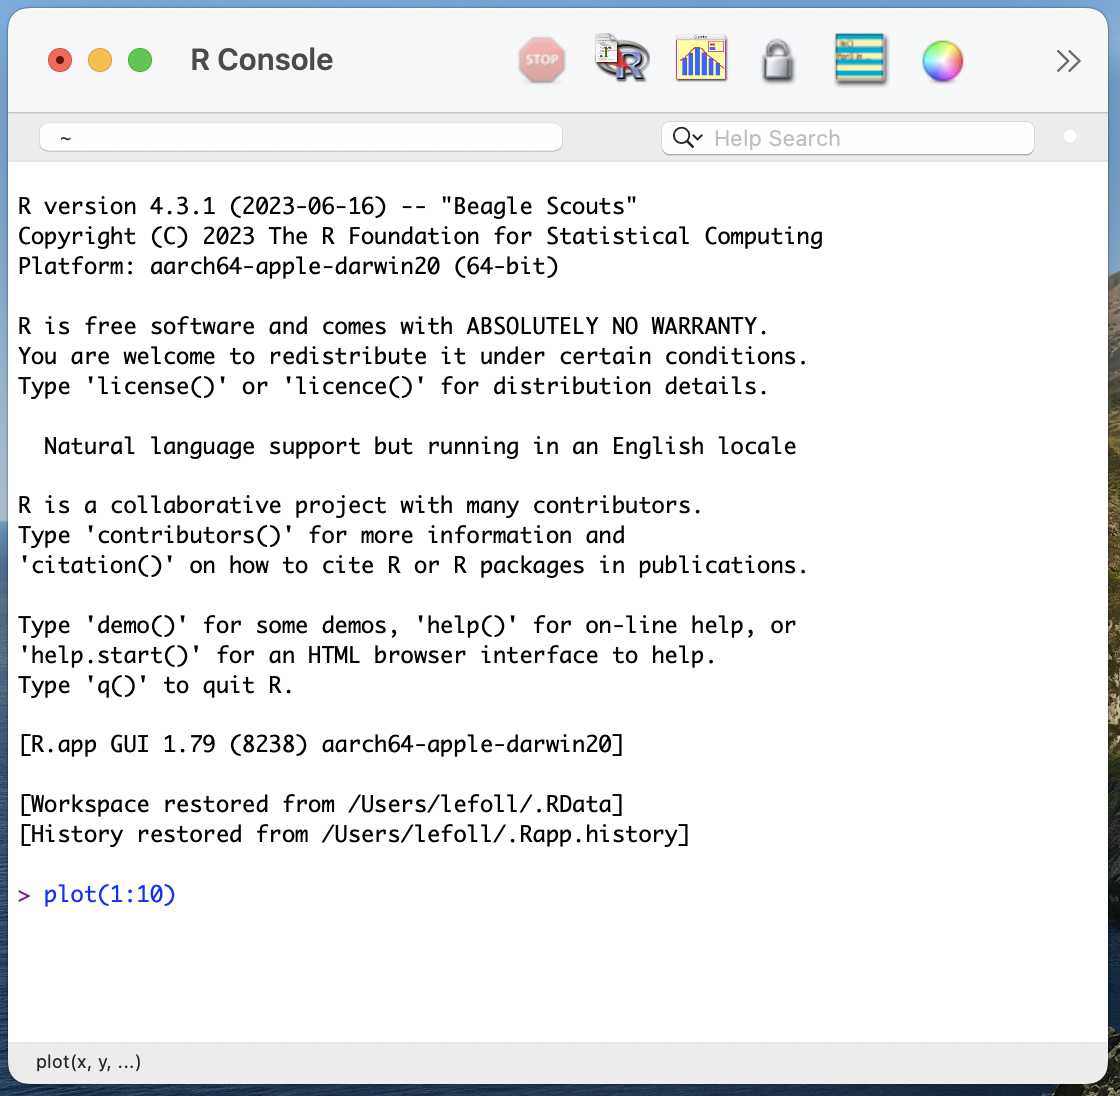
\includegraphics{images/RConsole.png}

}

\subcaption{\label{fig-console}Test command in R Console}

\end{minipage}%
%
\begin{minipage}{0.50\linewidth}

\centering{

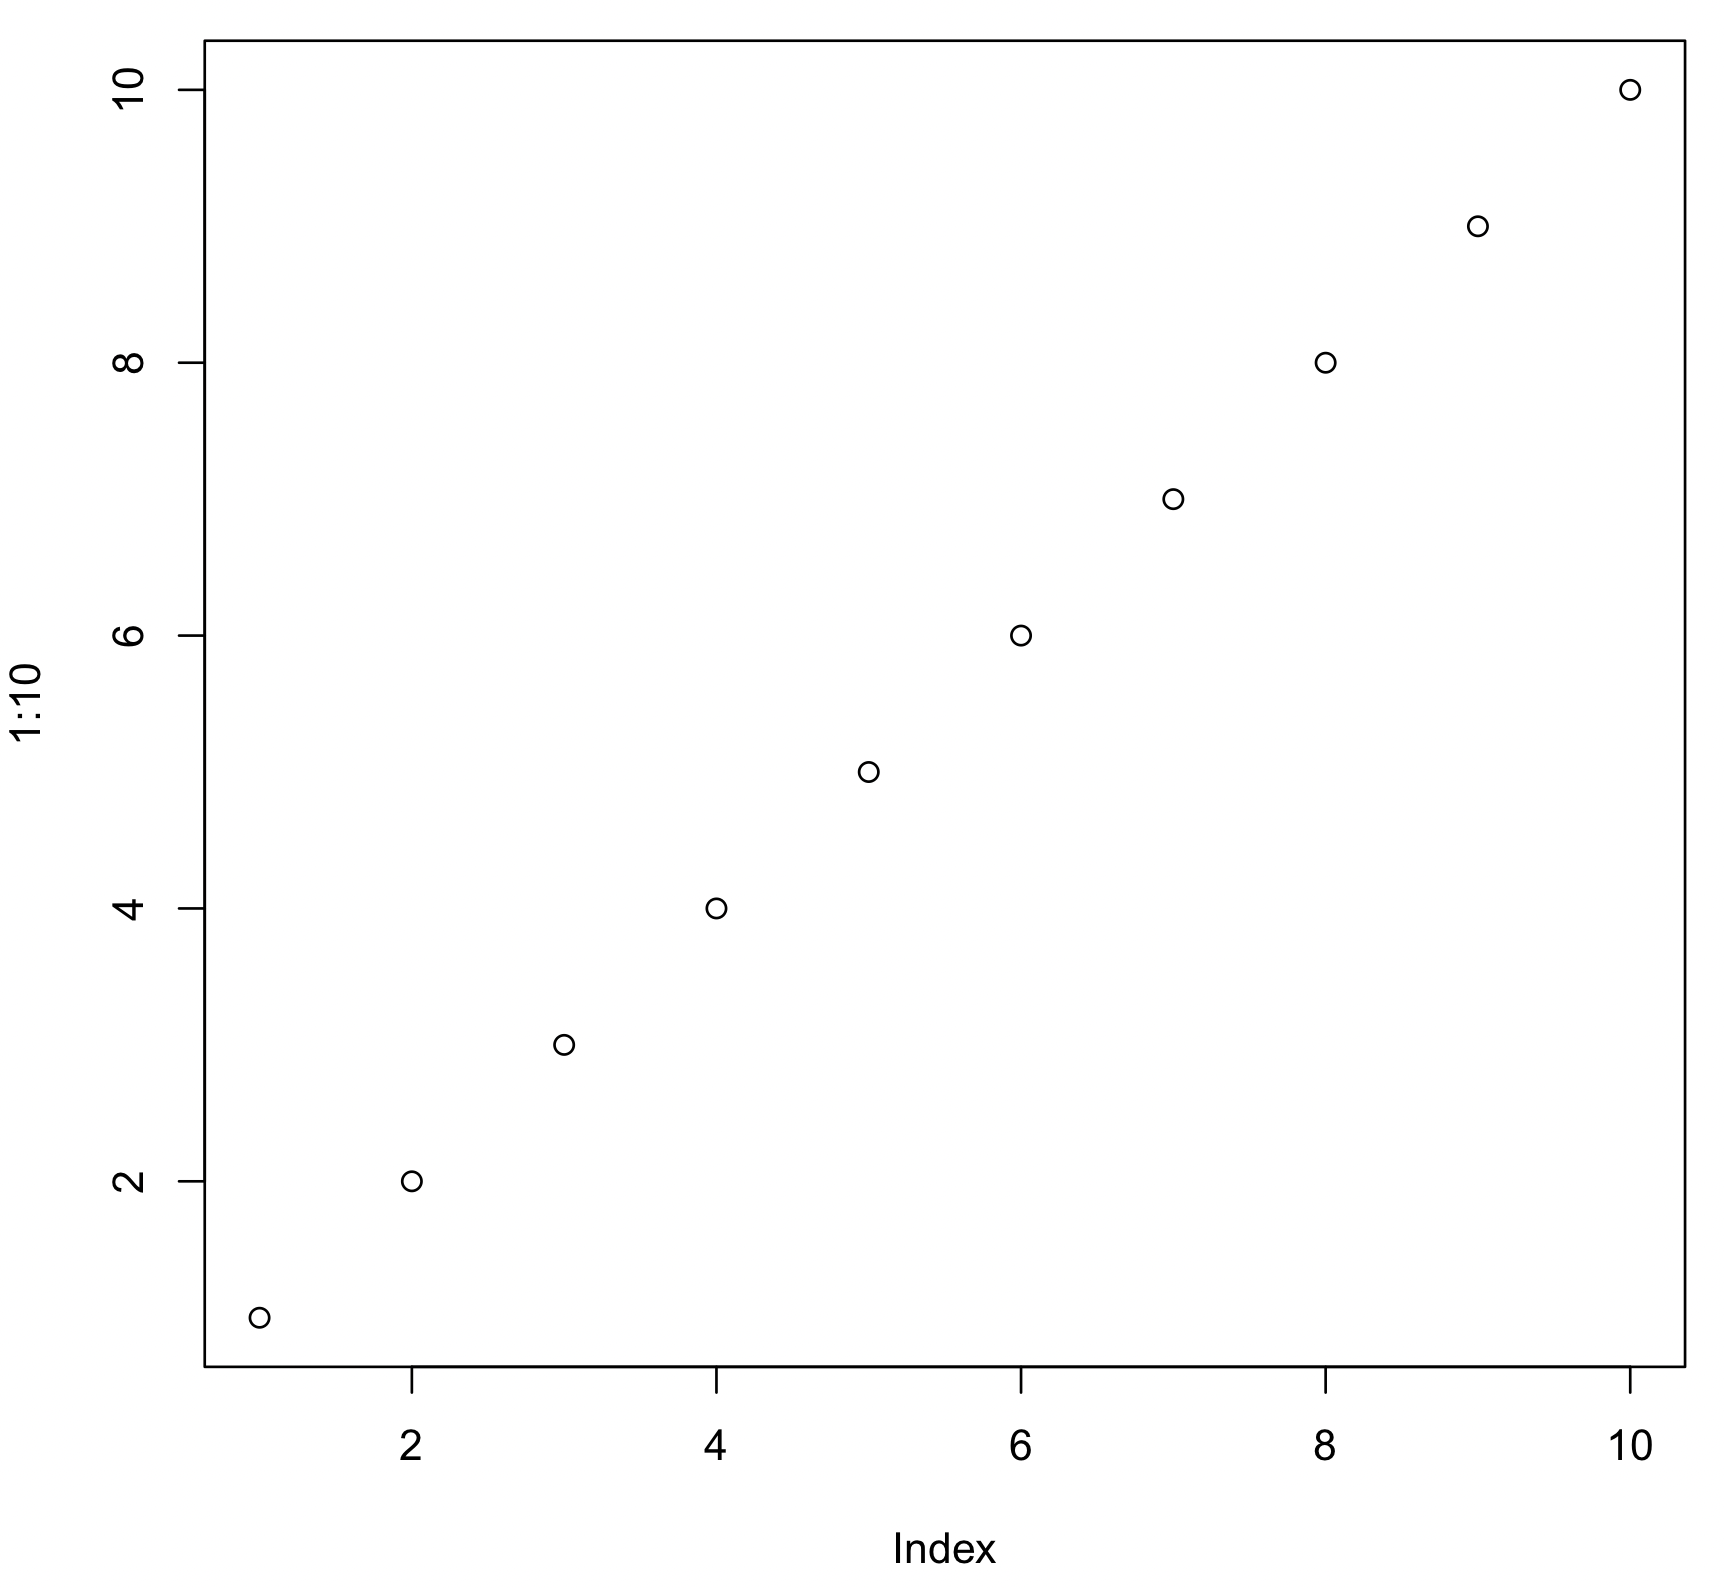
\includegraphics{images/TestingRPlot.png}

}

\subcaption{\label{fig-testplot}Resulting plot}

\end{minipage}%

\caption{\label{fig-Rtest}Testing R}

\end{figure}%

✅ If you see the plot above, you have successfully installed and tested
\texttt{R} and you can go on to installing \texttt{RStudio}.

⚠️ If that's not the case, make a note of the errors produced (copy and
paste them into a text document or take a screenshot) and search for
solutions on the Internet. It is very likely that many other people have
already encountered the same problem as you and that someone from the
\texttt{R} community has posted a solution online.

\subsubsection{\texorpdfstring{How to install
\texttt{RStudio}:}{How to install RStudio:}}\label{how-to-install-rstudio}

Visit RStudio's website
(https://www.rstudio.com/products/rstudio/download/) to download RStudio
Under the column called ``RStudio Desktop FREE'', click ``Download''
Find your operating system (Mac, Windows, or Linux) Select the ``latest
release'' on the page for your operating system Download and install the
application

\begin{verbatim}

If you do have issues, consider the Data Carpentry page (https://datacarpentry.org/R-ecology-lesson/) and then reach out for help. Another excellent place to get help is the RStudio Community forums (https://community.rstudio.com/).

### Setting up RStudio

Now that we’ve installed both R and RStudio, we will be accessing R through RStudio. One of the most reliable ways to tell if you’re opening R or RStudio is to look at the icons: R Icon and RStudio Icon

Figure 5.1: Icons

Whenever we want to work with R, we’ll open RStudio. RStudio interfaces directly with R, and is an Integrated Development Environment (IDE). This means that RStudio comes with built-in features that make using R a little easier. If you’d like more information on the difference between R and RStudio, we recommend the “Getting Started” section of the Modern Dive (https://moderndive.com/1-getting-started.html#) textbook (Ismay & Kim, 2019).

You do not have to use RStudio to access R, and many people don’t!

Other IDEs that work with R include:
\end{verbatim}

Jupyter notebook (https://jupyter.org/) VisualStudio
(https://visualstudio.microsoft.com/services/visual-studio-online/) VIM
(https://github.com/jalvesaq/Nvim-R) IntelliJ IDEA
(https://plugins.jetbrains.com/plugin/6632-r-language-for-intellij)
EMACS Speaks Statistics (ESS) (https://ess.r-project.org/)

\begin{verbatim}

This is a non-exhaustive list, and most of these options require a good deal of familiarity with a given IDE. We bring up alternative IDEs—particularly ESS—because RStudio, as of this writing, is not fully accessible for learners who utilize screen readers. We have chosen to use RStudio in this text in order to standardize the experience, but we encourage you to choose the IDE that best suits your needs!

### RStudio layout

When we open RStudio for the first time, we should see something similar to this: RStudio Default Layout with console, environment, and files

Figure 5.2: RStudio Layout

We’ll refer to these three “panes” as the “Console pane”, the “Environment pane”, and the “Files pane”. The large square on the left is the Console pane, the square in the top right is the Environment pane, and the square in the bottom right is the Files pane.

As you work with R more, you’ll find yourself using the tabs within each of the panes.

When we create a new file, such as an R script, an R Markdown file, or a Shiny app, RStudio will open a fourth pane, known as the “source pane”. The source pane should show up as a square in the top left. We can open up an .R script in the source pane by going to “File”, selecting “New File”, and then selecting “R Script”: Creating a New Script in RStudio by going to file then R script

Figure 5.3: Creating a New R Script in RStudio

You do not need to do anything specific with this file, but we encourage you to experiment with it if you would like! 5.5.2 Customizing RStudio

One of the balances we’ve tried to strike in this text is a balance between best practices in your workflow (how you’ll use R in your projects) and your R code. A best practice for your workflow is to ensure that you’re starting with a blank slate every time you open R (through RStudio). To accomplish this, go to “Tools”, and select “Global Options” from the dropdown menu. Selecting Global Options from the Tool Dropdown Menu

Figure 5.4: Selecting Global Options from the Tool Dropdown Menu

The “General” tab will open, with several checkboxes selected and unselected. The most important thing you can do is select “Never” next to the “Save workspace to .RData on exit:” prompt. After selecting “Never”, go through and check and uncheck boxes so that your General tab looks like this: General tab from the Global Options in RStudio

Figure 5.5: General Tab from Global Options

Last, but certainly not least, click on the “Appearance” tab from within Global Options. From here you can select your RStudio Font, Font Size, and Theme. Go through the options and select an appearance that works best for you, and know that you can always come back and change it! 5.5.3 Minimized and missing panes

If, at any point, you find that one of your panes seems to have “disappeared”, one of two things has likely happened:
\end{verbatim}

A pane has been minimized A pane has been closed

\begin{verbatim}

Let’s look at the Environment pane as an example. If the Environment pane has been minimized, we’ll see something like this: RStudio layout with a minimized Environment Pane

Figure 5.6: RStudio Layout with the Environment Pane Minimized

We know that the Environment pane has been minimized because although we can see the pane headers in the top right, we can’t see the information within the Environment pane. To fix this, we can click on the icon of two squares in the top right of the Environment pane. If you click on the icon of the large square in the top right of the Environment pane, you’ll maximize the Environment pane and minimize the Files pane. We do not want to do this, since we would prefer to see all the panes at once.

If the Environment pane has somehow been closed, you can recover it by going to the “View” menu, selecting “Panes”, and then selecting “Pane Layout”, like so: Accessing the Pane Layout from the View Dropdown Menu

Figure 5.7: Accessing the Pane Layout from the View Dropdown Menu

When we select Pane Layout, we’ll see this: Pane Layout Options within RStudio

Figure 5.8: Pane Layout Options within RStudio

From here, you can select which tabs you’d like to appear within each pane, and you can even change where each pane appears within RStudio. If our Environment Pane had been closed, we would select it from the Pane Layout in order to re-open it within RStudio. 5.6 Writing and running code in RStudio

Up to this point, we’ve been exploring the RStudio interface and setting up our preferences. Now, we’ll shift to some basic coding practices. In order to run code in R, you need to type your code either in the Console or within an .R script.

We generally recommend creating an .R script as you’re learning, as it allows you to type all of your code, add comments, and then save your .R script for reference. If you work entirely in the Console, anything that you type in the Console will disappear as soon as you restart or close R, and you will not be able to reference it in the future.

### Writing code in the console

To run code in the Console, you type your code next to the \> and hit Enter. We’ll spend a little time practicing running code in the Console by exploring some basic properties of coding in R.

In the Console, type 3 + 4 and hit Enter. You should see the following: Adding 3 and 4 on the console

Figure 5.9: Using the Console as a Calculator

We’ve just used R to add the numbers 3 and 4. R has returned the sum of 3 + 4 on a new line, next to \[1\]. The \[1\] tells us that there is one row of data.

We can also use R to print out text. Type the following in the Console and hit Enter:

print("I am learning R")

We should see this in the Console: Printing I am learning R on the console

Figure 5.10: Printing Text to the Console

There’s one error that you’re likely going to come across, both when running code in the Console as well as in an R script. Let’s explore that error now by running the following code in the Console and hitting Enter:

print("This is going to cause a problem"

Make sure that you left off the closing parenthesis! What you’ll see in the Console is: Printing this is going to cause a problem with the last parantheses missing

Figure 5.11: Incomplete Parentheses Change What R Expects Next

When we’re missing a closing parenthesis, R is expecting us to provide more code. We know this because instead of seeing a carat \> in our Console, we see a +, and R has not returned the print statement that we were expecting! There are two ways to fix this problem:
\end{verbatim}

Type the closing ) in the Console and hit Enter Hit the Esc key ```

Go ahead and run this intentional error, and try each of the options
above. Compare the output of each, and think about how they're
different. Can you think of when you might want to use one option
instead of the other? 5.6.2 Writing code in an R script

There are three main ways to run code in an .R script: - Highlight the
line(s) of code you'd like to run and press Ctrl + Enter - Highlight the
line(s) of code you'd like to run and click the ``Run'' button in the R
script pane - To run every line of code in your file you can press Ctrl
+ Shift + Enter

Create a new .R script, or open the one you created earlier in this
chapter. Next, type in the following code and run it using each of the
options listed above.

print(``We're going to use R as a calculator.'') print(``First up,
addition!'') 12 + 8 632 + 41 print(``Next, subtraction!'') 48 - 6 0.65 -
1.42

Feel free to spend some more time writing and running code within your
.R script, or move on to the next section, where we'll add comments to
our code. 5.6.3 Commenting your code in R

It is considered good practice to comment your code when working in an
.R script. Even if you are the only person to ever work on your code, it
can be helpful to write yourself notes about what you were trying to do
with a specific piece of code. Moreover, writing comments in your code
as you work through the examples in this book is a great way to help
reinforce what you're learning. Comments are ignored by R when running a
script, so they will not affect your code or analysis.

To comment out a line of code, you can place a pound sign (also called
an octothorpe!) \# in front of the line of code that you want to exclude
when you're running your script. Be careful when excluding certain lines
of code, especially in longer files, as it can be easy to forget where
you've commented out code. It is often better to simply start a new
section of code to tinker with until you get it working as expected,
rather than commenting out individual lines of code.

We can also write comments in line with our code, like this:

\#' this will be a short code example. \#' you are not expected to know
what this does, \#' nor do you need to try running it on your computer.
library(readr) \# load the readr package library(here) \# load the here
package data \textless- read\_csv(here(``file\_path'',
``file\_name.csv'')) \# save file\_name.csv as data

If you think you'll be writing more than one line of comments, you can
do a pound sign followed by a single quotation mark (\#`). This will
continue to comment out lines of text or code each time you hit Enter.
You can delete the \#' on a new line where you want to write code for R
to run. This method is useful when you're writing a long description of
what you're doing in R.

Note: when we refer to ``commenting'' we're referring to adding in
actual text comments, whereas ``commenting out'' refers to using the
pound sign (octothorpe) in front of a line of code so that R ignores it.
We will also use the phrase ``uncomment code'', which means you should
delete (or omit when typing out) the \# or \#' in an example.

\subsection{Functions introduced}\label{functions-introduced}

For the ``functions introduced'' sections, you will notice that some
look a little bit different than others. For example,
devtools::install\_github() is different than install.packages().

The reason is that the install\_github() function comes from a specific
package (which we'll discuss in great depth in this and the following
chapter). If you had a hunch that this function comes from the devtools
package, then you'd be correct. The :: symbols (described more in
Chapter 6) mean that a specific function comes from a particular
package, something that we wanted to point out so that you will know
which package you will need to use if you want to use the function. Not
sure what some of these terms mean quite yet? Read on in this chapter to
learn more about installing and using packages! ```

install.packages() devtools::install\_github() library() print()
readr::read\_csv() here::here() swirl::swirl() swirl::install\_course()
```

\subsection{Exploring R with the \{swirl\}
package}\label{exploring-r-with-the-swirl-package}

If you were able to install the \{dataedu\} package without any issues
or concerns and you're eager to get started exploring everything that R
can do, you can supplement your learning through \{swirl\}
(https://swirlstats.com/students.html).

You can install \{swirl\} by running the following code:

install.packages(``swirl'')

\{swirl\} is a set of packages (see more on packages in Chapter 6) that
you can download, providing an interactive method for learning R by
using R in the RStudio Console. Since you've already installed R,
RStudio, and the \{swirl\} package, you can follow the instructions on
the \{swirl\} webpage or run the following code in your Console pane to
get started with a beginner-level course in \{swirl\}:

library(swirl) install\_course(``R\_Programming\_E'') swirl()

There are multiple courses available on \{swirl\}, and you can access
them by installing them and then running the swirl() command in your
console. We are not affiliated with \{swirl\} in any way, nor is
\{swirl\} required to progress through this text, but it's a great
resource that we want to make sure is on your radar!

\subsection{Conclusion}\label{conclusion}

Congratulations! At this point in the book, you've installed R and
RStudio, explored the RStudio IDE, and even written some basic code. At
this point, you're set up to either move on to Chapter *, where we'll do
a deeper dive into projects, packages, and functions, and how those
relate to your future data tasks. We will also introduce help
documentation and some skills for when you're working with new or
unfamiliar information. If that all sounds familiar to you already, you
can jump ahead to a walkthrough of your choosing!

\bookmarksetup{startatroot}

\chapter*{References}\label{references}
\addcontentsline{toc}{chapter}{References}

\markboth{References}{References}

\phantomsection\label{refs}
\begin{CSLReferences}{1}{0}
\bibitem[\citeproctext]{ref-LibreOffice2024}
2024. LibreOffice. \emph{Wikipedia}.
\url{https://en.wikipedia.org/w/index.php?title=LibreOffice&oldid=1218520104}.

\bibitem[\citeproctext]{ref-parsonsCommunitysourcedGlossaryOpen2022}
Parsons, Sam, Flávio Azevedo, Mahmoud M. Elsherif, Samuel Guay, Owen N.
Shahim, Gisela H. Govaart, Emma Norris, et al. 2022. A community-sourced
glossary of open scholarship terms. \emph{Nature Human Behaviour}.
Nature 6(3). 312--318. \url{https://doi.org/10.1038/s41562-021-01269-4}.

\end{CSLReferences}

\cleardoublepage
\phantomsection
\addcontentsline{toc}{part}{Appendices}
\appendix

\chapter{Next-step resources}\label{next-step-resources}

In the hope that this textbook has inspired you to dive deeper into the
wonderful world of quantitative data analysis, statistics, data
visualisation, and coding in R, here is a (work-in-progress) curated
list of further resources to continue your learning journey! 🚀✨

\section{Recommended resources specific to the language
sciences}\label{recommended-resources-specific-to-the-language-sciences}

\begin{itemize}
\item
  Brezina, Vaclav. 2018. Statistics in Corpus Linguistics: A Practical
  Guide. Cambridge: Cambridge University Press.
  https://doi.org/10.1017/9781316410899.
\item
  Desagulier, Guillaume. 2017. Corpus Linguistics and Statistics with R:
  Introduction to Quantitative Methods in Linguistics (Quantitative
  Methods in the Humanities and Social Sciences). Cham: Springer
  International Publishing.
\item
  Gries, Stefan Thomas. 2013. Statistics for linguistics with R: a
  practical introduction. 2nd revised edition. Berlin: De Gruyter
  Mouton.
\item
  LADAL contributors. Tutorials of the Language Technology and Data
  Analysis Laboratory. \url{https://ladal.edu.au/tutorials.html}
  \texttt{Open\ Educational\ Resource}.
\item
  Levshina, Natalia. 2015. How to do linguistics with R: Data
  exploration and statistical analysis. Amsterdam: John Benjamins.
\item
  Schneider, Dr Gerold \& Max Lauber. 2020. Statistics for Linguists.
  \url{https://dlf.uzh.ch/openbooks/statisticsforlinguists/}
  \texttt{Open\ Educational\ Resource}.
\item
  Winter, Bodo. 2019. Statistics for Linguists: An Introduction Using R.
  New York: Routledge.
  \href{https://doi.org/10.1017/9781316410899}{https://doi.org/10.4324/9781315165547}.
\end{itemize}

\section{Further Open Educational Resources (in no particular
order)}\label{further-open-educational-resources-in-no-particular-order}

\begin{itemize}
\tightlist
\item
  Diez, David, Mine Cetinkaya-Rundel, Christopher Barr \& OpenIntro.
  2015. OpenIntro Statistics. Leanpub. \url{https://leanpub.next/os}.
\item
  Guide to Effect Sizes and Confidence Intervals:
  \url{https://matthewbjane.quarto.pub/guide-to-effect-sizes-and-confidence-intervals/}
\item
  Happy Git and GitHub for the useR: \url{https://happygitwithr.com/}
\item
  Quarto \& reproducibility:
  \url{https://ucsbcarpentry.github.io/Reproducible-Publications-with-RStudio-Quarto/index.html}
\item
  Modern Data Visualization with R:
  \url{https://rkabacoff.github.io/datavis}
\item
  Building reproducible analytical pipelines with R:
  \url{https://raps-with-r.dev/}
\item
  Modern Plain Text Computing:
  \url{https://mptc.io/content/01-content.html}
\item
  \url{https://www.data-to-viz.com/}
\item
  Interpreting data visualisation:
  \url{https://pressbooks.library.torontomu.ca/criticaldataliteracy/}
\item
  Improve your statistical inferences:
  \url{https://lakens.github.io/statistical_inferences/}
\item
  What they forgot to teach you about R: \url{https://rstats.wtf/}
\item
  Introduction to Data Science:
  \url{https://florian-huber.github.io/data_science_course/book/cover.html}
\item
  Data Science in Education Using R:
  \url{https://datascienceineducation.com/}
\item
  Models Demystified: A Practical Guide from t-tests to Deep Learning
  \url{https://m-clark.github.io/book-of-models/}
\item
  Data Visualization in R
  \url{https://datavizf23.classes.andrewheiss.com/}
\item
  R for Data Science \url{https://r4ds.hadley.nz/intro}
\end{itemize}



\end{document}
